\documentclass[a5paper,oneside]{amsart}
\usepackage[scale={.9,.9}]{geometry}
\usepackage{mathrsfs}
\usepackage{ stmaryrd }
\usepackage{ dsfont }
\usepackage{ amssymb }
\usepackage{ upgreek }
\usepackage{ color }
\usepackage{graphicx}
\theoremstyle{plain}
\newtheorem{theorem}{Theorem}
\newtheorem{lemma}{Lemma}
\newtheorem{corollary}{Corollary}
\newtheorem{proposition}{Proposition}
\newtheorem{conjecture}{Conjecture}
\theoremstyle{definition}
\theoremstyle{solucion}
\newtheorem{problema}{Problema}
\newtheorem*{definition}{Definition}
\newtheorem*{remark}{Remark}
\title[Problemas de Procesos I]{Problemas de Procesos Estoc\'asticos I\\ Semestre 2013-II\\ Posgrado en Ciencias Matem\'aticas\\ Universidad Nacional Aut\'onoma de M\'exico \\ TAREA 1}
\author{\textcolor[rgb]{0.5,0.5,1}{Antonio Soriano Flores}}
%\address{act_antonio@hotmail.com}
\usepackage[colorlinks,citecolor=blue,urlcolor=blue]{hyperref}
%\setlength{\textwidth}{17.2cm} % was 18.2
%\setlength{\textheight}{23cm} % was 23
%\setlength{\torgin}{-1cm} % was 0
%\setlength{\oddsidemargin}{-0.6cm}
%\setlength{\evensidemargin}{-0.6cm}

%\setlength{\textwidth}{18.9cm} % was 18.2
%\setlength{\textheight}{26.73cm} % was 23
%\setlength{\topmargin}{1cm} % was 0
%\setlength{\oddsidemargin}{0cm} %
%\setlength{\evensidemargin}{.8cm}
%% Arreglar pues ahora utilizas papel A4.

%Operadores

\DeclareMathOperator{\ivp}{IVP} %
\DeclareMathOperator{\sgn}{sgn} %
\DeclareMathOperator{\md}{mod}
\DeclareMathOperator{\ima}{Im}%
\DeclareMathOperator{\id}{Id} %
\DeclareMathOperator{\homo}{Hom} %
\DeclareMathOperator{\inter}{Int}
\DeclareMathOperator*{\Lim}{lim}
\DeclareMathOperator*{\Limsup}{lim\ sup}
\DeclareMathOperator*{\Liminf}{lim\ inf}
\DeclareMathOperator*{\Min}{m\text{\ii}n}
\DeclareMathOperator{\Aff}{Aff}
\DeclareMathOperator{\Affb}{\overline{\Aff}}
\DeclareMathOperator{\sdfd}{dfd}
\DeclareMathOperator{\scdfd}{dfd}
\DeclareMathOperator{\Beta}{B}
\DeclareMathOperator{\pd}{PD}
\DeclareMathOperator{\supp}{supp}
\DeclareMathOperator{\diam}{diam}
\newcommand{\ind}{\operatornamewithlimits{\perp}}
\DeclareMathOperator{\av}{Abs}
\DeclareMathOperator{\cb}{CB}
\DeclareMathOperator{\cbi}{CBI}
\DeclareMathOperator{\gwi}{GWI}
\DeclareMathOperator{\gw}{GW}
\newcommand{\rtree}{$\re$\nbd tree}
\newcommand{\leb}{\text{Leb}}
%Notaci�n



%Delimitadores
\newcommand{\ceil}[1]{\ensuremath{\lceil #1 \rceil}}
%\renewcommand{\floor}[1]{\ensuremath{\lfloor #1 \rfloor}}

%Formato
\newcommand{\defin}[1]{{\bf #1}}
\newcommand{\mc}[1]{\ensuremath{\mathscr{#1}}}
\newcommand{\bb}[1]{\mathbb{#1}}


%Notation

\newcommand{\card}[1]{\ensuremath{\left| #1 \right|}}
\newcommand{\lccb}{LCCB}
\newcommand{\pss}{S}
\newcommand{\compact}{K}
\newcommand{\psm}{\rho}
\newcommand{\ps}{\paren{\pss,\psm}}
\newcommand{\pse}{x}
\newcommand{\psep}{y}
\newcommand{\psepp}{z}
\newcommand{\saps}{\B_{\pss}}
\newcommand{\bre}{\B_{\re}}
\newcommand{\sko}{D}
\newcommand{\trees}{T}
\newcommand{\C}{C}
\newcommand{\refm}{\mu}
\newcommand{\den}{p}
\newcommand{\psd}[1]{\mc{P}_{#1}}
\newcommand{\s}{\ensuremath{\sigma}}
\newcommand{\bden}{M}
\newcommand{\hh}[1]{{\bf H#1}}
\newcommand{\ball}[2]{\imf{B_{#1}}{#2}}
\newcommand{\mmc}[1]{\imf{\tilde\omega}{#1}}
\newcommand{\rg}[1]{\ensuremath{\imf{\mathbb{G}}{#1}}}




\newcommand{\dfd}{\ensuremath{\stackrel{\sdfd}{=}}}
\newcommand{\deq}{\ensuremath{\stackrel{d}{=}}}

\newcommand{\ley}[2]{\ensuremath{\imf{\mc{L}^{#2}}{#1}}}
\newcommand{\leyc}[3]{\ensuremath{\imf{\mc{L}^{#3}}{#1\left|#2\right.}}}
\newcommand{\cond}[2]{\left.\vphantom{#2}#1\ \right| #2}

\newcommand{\e}{\ensuremath{\mathbf{e}}}
\newcommand{\esf}{\ensuremath{\mc{S}^{\downarrow}}}
%\newcommand{\ps}[1]{\mathscr{P}\paren{#1}}
\newcommand{\fun}[3]{\ensuremath{#1:#2\to #3}}
\newcommand{\fund}[3]{\ensuremath{#1:#2\mapsto #3}}
\newcommand{\set}[1]{\ensuremath{\left\{ #1\right\} }}
\newcommand{\sets}[1]{\ensuremath{{\mathbf #1}}}
\newcommand{\paren}[1]{\ensuremath{\left( #1\right) }}
\newcommand{\bra}[1]{\ensuremath{\left[ #1\right] }}
\newcommand{\seq}[1]{\ensuremath{ #1 _1,\ldots ,#1 _n }}
\newcommand{\sm}[3]{\left[ #1\right]_{#2}^{#3}}
\newcommand{\cde}{\Rightarrow}
\newcommand{\cdfd}{\ensuremath{\stackrel{\scdfd}{\cde}}}
\newcommand{\convo}[2]{\ensuremath{#2^{\!* #1}}}

\newcommand{\tl}[1]{\ensuremath{\hat{#1}}}

\newcommand{\matt}[3]{#1_{#2\, #3}}
\newcommand{\sip}{\bb{P}}
\newcommand{\jump}[2]{\ensuremath{\Delta #1_{#2}}}
\newcommand{\cadlag}{c\`adl\`ag}
\newcommand{\se}{\ensuremath{\bb{E}}}
\newcommand{\ssa}{\ensuremath{\mathscr{F}}}
\newcommand{\si}{{\ensuremath{\bf{1}}}}
\newcommand{\sbr}{\ensuremath{\mc{B}_{\re}}}
%\newcommand{\siind}{\ensuremath{\perp}}
\newcommand{\sigam}{\ensuremath{\Gamma}}
\newcommand{\smc}{\ensuremath{m}}
\newcommand{\sfleche}{S^{\downarrow}_f}

\newcommand{\gafun}[1]{\sigam \paren{#1}}
\newcommand{\poi}[1]{\ensuremath{\mc{P}\!_{#1}}}
\newcommand{\ber}[1]{\ensuremath{\mc{B}\!_{#1}}}
\newcommand{\fcpoi}[1]{\ensuremath{\hat{\mc{P}}\!_{#1}}}
%\newcommand{\ind}{\siind}
\newcommand{\condind}[3]{\ensuremath{#1\ind_{#3}#2}}
\newcommand{\sig}[1]{$\sigma$-\nobreakdash #1}
\newcommand{\sa}{\ensuremath{\sigma}\nbd field}
\newcommand{\realtree}{\ensuremath{\re}\nbd tree}
\newcommand{\eps}{\ensuremath{ \varepsilon}}
\newcommand{\na}{\ensuremath{\mathbb{N}}}
\newcommand{\en}{\ensuremath{\mathbb{Z}_+}}
\newcommand{\eti}{\ensuremath{\mc{U}}}
\newcommand{\etic}{\ensuremath{\mathbb{U}}}
\newcommand{\z}{\ensuremath{\mathbb{Z}}}
\newcommand{\re}{\ensuremath{\mathbb{R}}}
\newcommand{\ra}{\ensuremath{\mathbb{Q}}}
\newcommand{\com}{\ensuremath{\mathbb{C}}}
\newcommand{\con}[1]{\ensuremath{\overline{#1}}}
\newcommand{\proba}[1]{\ensuremath{\sip\! \left( #1 \right)}}
\newcommand{\probas}[2]{\ensuremath{#1\! \left( #2 \right)}}
\newcommand{\probac}[2]{\ensuremath{\sip\! \left( #1 \, | #2 \right)}}
\newcommand{\esp}[1]{\ensuremath{\se\! \left( #1 \right)}}
%\newcommand{\espc}[2]{\ensuremath{\se\! \left( #1 | #2 \right)}}
\newcommand{\espc}[2]{\ensuremath{\imf{\se}{\cond{#1}{#2}}}}
\newcommand{\var}[1]{\ensuremath{\text{Var}\! \left( #1 \right)}}
\newcommand{\cov}[1]{\ensuremath{Cov\! \left( #1 \right)}}
\newcommand{\abs}[1]{\hspace{.25mm}\left|#1\right|\hspace{.25mm}}
\newcommand{\ila}[2]{\ensuremath{\int #1\, d#2}}
\newcommand{\ilas}[3]{\ensuremath{\int_{#1} #2\, d#3}}
\newcommand{\il}[3]{\ensuremath{\int #1\, \imf{#2}{d#3}}}
\newcommand{\is}[4]{\ensuremath{\int_{#1} #2\, \imf{#3}{d#4}}}
\newcommand{\lp}[2]{\ensuremath{\mc{L}_#1\!\paren{#2} }}
\newcommand{\lpc}[4]{\ensuremath{\mc{L}_#1\!\paren{ #2 , #3 , #4 }}}
\newcommand{\ip}[1]{\ensuremath{\int #1\, d\sip }}
\newcommand{\ips}[2]{\ensuremath{\int_{#1} #2\, d\sip}}
\newcommand{\F}{\ssa}
\newcommand{\uF}{\ssa^u}
\newcommand{\G}{\ensuremath{\mc{G}}}
\newcommand{\h}{\ensuremath{\mc{H}}}
\newcommand{\B}{\ensuremath{\mc{B}}}
\newcommand{\f}[1]{\ssa_{#1}}
\newcommand{\fx}[2]{\ssa_{#1}^{#2}}
\newcommand{\indi}[1]{\si_{#1}}
\newcommand{\imi}[2]{#2^{-1}\!\paren{#1}}
\newcommand{\ooo}{\ensuremath{ \omega  } }
\newcommand{\oo}{\ensuremath{ \Omega  } }
\newcommand{\p}{\ensuremath{ \sip  } }
\newcommand{\q}{\ensuremath{ \bb{Q}  } }
\newcommand{\ofp}{\ensuremath{ \paren{ \Omega ,\F ,\p } } }
\newcommand{\med}[2]{\ensuremath{\paren{#1}{#2}}-medible}
\newcommand{\vat}{\ensuremath{\fun{X}{\oo}{\re}}\ }
\newcommand{\pix}[1]{\ensuremath{\sip}_{\! #1}}
\newcommand{\px}[2]{\ensuremath{\sip_{\! #1}\!\paren{#2}}}
\newcommand{\pxc}[3]{\ensuremath{\sip_{\! #1}\!\left( #2 | #3 \right)}  }
\newcommand{\br}{\sbr}
\newcommand{\sag}[1]{\sigma\!\paren{#1}}
\newcommand{\cs}[1]{\ensuremath{#1}-p.s.}
\newcommand{\ore}{ \ensuremath{\overline{\re}}}
\newcommand{\fungen}[1]{\ensuremath{\varphi_{#1}}}%Comando para la notaciÛn de funciÛn generadora.
\newcommand{\cbin}[2]{\ensuremath{\paren{\begin{array}{c}#1\\#2\end{array}}}}
\newcommand{\fa}[2]{\ensuremath{{#1}^{\paren{#2}}}}
\newcommand{\dnor}[2]{\ensuremath{N(#1,#2)}}
\newcommand{\mb}{movimiento browniano}
\newcommand{\moc}[3]{\smc^{#3}(#1,#2)}
\newcommand{\clo}[1]{\ensuremath{\overline{#1}}}
\newcommand{\inte}[1]{\ensuremath{\inter #1}}
\newcommand{\fro}[1]{\ensuremath{\partial\paren{ #1}}}
\newcommand{\cd}[2]{\ensuremath{#1\stackrel{\mc{D}}{\to}#2}}
\newcommand{\pr}[3]{\ensuremath{#1_{#2}\!\paren{#3}}}
\newcommand{\oi}[1]{\ensuremath{\mc{O}\paren{#1}}}
\newcommand{\mw}{\ensuremath{\mathbb{P}}}
\newcommand{\me}{\ensuremath{\pi}}


\newcommand{\nbd}{\nobreakdash -}
\newcommand{\ii}{\'{\i}}
\newcommand{\n}{\~n}
\newcommand{\imf}[2]{\ensuremath{#1\!\paren{#2}}}
\newcommand{\floor}[1]{\ensuremath{\lfloor #1\rfloor}}
\newcommand{\proint}[2]{\ensuremath{\langle #1,#2\rangle}}
\newcommand{\vp}{\ensuremath{\varphi}}
\newcommand{\noru}[1]{\ensuremath{\|#1\|}}
\newcommand{\gen}[1]{\ensuremath{|#1 |}}
\newcommand{\vc}[1]{\ensuremath{\langle #1\rangle}}
\newcommand{\pc}[2]{\ensuremath{\langle#1,#2\rangle}}
\newcommand{\vcd}[1]{\ensuremath{\left[#1\right]}}

\newcommand{\sml}{\ensuremath{\nu}}
\newcommand{\ml}[1]{\ensuremath{\imf{\sml}{#1}}}
\newcommand{\va}[2]{\ensuremath{\imf{V_{#1}}{#2}}}
\newcommand{\clase}[1]{\ensuremath{\mc{C}^{#1}}}
\newcommand{\marte}[2]{\ensuremath{\imf{\mc{E}^{#2}}{#1}}}

\newcommand{\dencero}[1]{\ensuremath{\left. \frac{\partial }{\partial #1}\right|_{#1=0} }}
%\newcommand{\premin}[1]{\ensuremath{\stackrel{\leftarrow}{#1}}}
%\newcommand{\postmin}[1]{\ensuremath{\stackrel{\rightarrow}{#1}}}
\newcommand{\premin}[1]{\ensuremath{{#1}^{\leftarrow}}}
\newcommand{\postmin}[1]{\ensuremath{{#1}^{\rightarrow}}}



%Ambientes (Environments)

\newenvironment{esn}{\begin{displaymath}}{\end{displaymath}}
\newenvironment{ecn}{\begin{equation}}{\end{equation}}
\newenvironment{listeo}{\begin{list}{\alph{enumi})}{\usecounter{enumi}}}{\end{list}}
\newenvironment{numerai}{\begin{list}{\roman{enumi})}{\usecounter{enumi}}}{\end{list}}
%\usepackage[colorlinks,citecolor=blue,urlcolor=blue]{hyperref}
\begin{document}
\maketitle
\textcolor[rgb]{0.2,0.5,0.7}{
\begin{problema}
Sean $\paren{X_n}_{n\in\na}$ un proceso estoc\'astico con valores reales y $A\subset\re$ un boreliano. Pruebe que si\begin{esn}
T_0=0\quad\text{y}\quad T_{n+1}=\min\set{k>T_n: X_k\in A}
\end{esn}entonces $T_n$ es un tiempo de paro para toda $n$ y $T_n\to \infty$ puntualmente conforme $n\to\infty$. 
\end{problema}
}
\defin{Soluci\'on: }  Primero notemos que como no se nos dice cu\'al  es la filtraci\'on del proceso asumiremos que: 
$$
 \F_0=\set{\Omega,\emptyset}
 \F_n=\sigma\set{X_1\dotsb X_n} ,
$$

El caso   $T_0$   es f\'acil pues es constante y por tanto es medible para cualquier $\sigma$-\'algebra en part\'icular para $\F_0$ y por tanto
$\set{T_0=n}\in\F_0$  lo que implica que es tiempo de paro.

Ahora,  como  $T_1:=\min\set{k>0: X_k\in A}$  (El primer arribo al conjunto A) . Entonces el evento $\set{T_1=n}$  lo podemos expresar como:
$$
\set{T_1=n}=\set{X_1\notin A,X_2 \notin A,\dotsb,X_{n-1} \notin A, X_n \in A }=\set{\bigcap_{k=1}^{n-1}X_k\notin A} \cap \set{X_n \in A}
$$
De lo anterior como cada $X_k$ es $\F_k$-medible   $\paren{1 \leq k \leq n-1}$ y por ser $\F_n$ filtraci\'on implica que $ \set{\bigcap_{k=1}^{n-1}X_k\notin A}  \in \F_n$
y finalmente es claro que $\set{X_n \in A}  \in \F_n$ de donde concluimos que $\set{T_1=n} \in \F_n$.

Siguiendo con el paso inductivo, supongamos que $T_k$ es tal que $\set{T_k=n} \in \F_n  \forall n$  P.D. que  $\set{T_{k+1}=n} \in \F_n  \forall n$

Notemos que por definici\'on  $T_k \geq k$ por lo que  en nuestra prueba si $n \leq k $ entonces $\set{T_{k+1}=n} = \emptyset \in \F_n$. Supongamos entonces $n\geq k+1$. Expresamos al evento en cuesti\'on de forma conveniente:
$$
\set{T_{k+1}=n}=\bigcup_{r=k}^{n-1}\set{T_k=r; X_{r+1} \notin A, X_{r+2} \notin A ,\dotsb, X_{n-1} \notin A; X_n \in A} 
$$
Como:\\
\begin{itemize}

\item $\set{T_k=r} \in \F_r$ (Por hip\'otesis de inducci\'on)  y $k \leq r \leq n-1$ entonces  por la filtraci\'on  $\F_r \subseteq \F_n$ de donde concluimos que
$\set{T_k=r} \in \F_n$.

\item  $\set{X_{r+1} \notin A} \in \F_{r+1}, \set{X_{r+2} \notin A} \in \F_{r+2},\dotsb, \set{X_{n-1} \notin A} \in \F_{n-1} $ . Entonces por ser $\F_n$-filtraci\'on  
tendr\'iamos que:  $\set{X_{r+1} \notin A ,\dotsb, X_{n-1} \notin A} \in \F_n$

\item  $\set{X_n \in A} \in \F_n$   
\end{itemize}
Por los tres puntos anteriores queda claro entonces que $\set{T_{k+1}=n} \in \F_n \forall n$. Lo que termina la prueba por inducci\'on.

Con esto acabamos de probar que $T_n$ cumple con la propiedad  $\set{T_n=k} \in \F_k \forall n$ y $\forall k$. Formalmente para ser tiempo de paro hay que probar
que tambi\'en $T_n$ es variable aleatoria pero esto se sigue inmediatamente del hecho de que $\set{T_n=k} \in \F_k$ implica que $\set{T_n \leq k} \in \F_k$  lo cual es
valido para toda $k$ y por tanto es medible respecta a la sigma \'algebra que contiene a  la filtraci\'on $\F$.  Por lo tanto se sigue que en efecto $T_n$ es tiempo de paro.

Para terminar con el ejercicio hay que probar que puntualmente $T_n\rightarrow \infty$. Sin embargo esto se sigue del hecho de la definici\'on  de $T_n$ pues 
se tiene que $T_n(\omega) \geq n$ de donde tomando limite cuando $n \rightarrow \infty$ se concluye que $T_n(\omega)\rightarrow \infty$

\textcolor[rgb]{0.2,0.5,0.7}{
\begin{problema}[Lo que siempre tiene una posibilidad razonable de suceder lo har\'a; (casi seguramente)-- y pronto]
Suponga que \(T\) es un tiempo de paro tal que para alg\'un \(N\in\na\) y \(\varepsilon>0\) se tiene que para toda \(n\in\na\):
 $$
 \p (T\leq N+ n|\F_n)>\varepsilon \text{ casi seguramente}
 $$
Al verificar la descomposici\'on
 $$
\p (T>kN)= \p (T>kN,T>(k-1)N),
 $$pruebe por inducci\'on que para cada \(k=1,2,\ldots\):
 $$
\p (T>kN)\leq \paren{1-\eps}^k. 
 $$Pruebe que \( \esp{T}<\infty \).
\end{problema}
}

\defin{Soluci\'on: }  Primero verificamos las descomposici\'on 
 $$
\p (T>kN)= \p (T>kN,T>(k-1)N),
 $$
 
 La cual es v\'alida por el hecho de que $\set{T>kN}\subseteq \set{T>(k-1)N}$  por lo que interceptando dichos eventos se tiene la igualdad
 $\set{T>kN}\cap \set{T>(k-1)N}=\set{T>kN}$ y luego tomando  probabilidad en ambos lados se tiene el resultado.
 
 Probaremos por inducci\'on sobre k
 
\begin{itemize}
\item Para $k=1$. Utilizando la hip\'otesis $\p (T\leq N+ n|\F_n)>\varepsilon$ con n=0
$$
\p (T\leq N|\F_0)>\varepsilon \Rightarrow \p(T > N|\F_0)<1-\varepsilon \text{ casi seguramente} 
$$
$$
\esp{\mathds{1}_{T\leq N}|\F_0}>\varepsilon  \Rightarrow  \esp{\mathds{1}_{T > N}|\F_0}<1-\varepsilon \text{ casi seguramente} 
$$
Tomando esperanza en ambos lados de la igualdad.
$$
\esp{ \esp{\mathds{1}_{T > N}|\F_0}}<\esp{1-\varepsilon} \Rightarrow  \esp{\mathds{1}_{T > N}} <1-\varepsilon \Rightarrow \p(T > N)<1-\varepsilon 
$$
\item Suponga $\p (T>kN)\leq \paren{1-\eps}^k$ P.D. $\p (T>(k+1)N)\leq \paren{1-\eps}^{k+1}$\\
Como:
$$\
\p (T>(k+1)N)=\p(T>(k+1)N,T>kN)=\esp{\mathds{1}_{\set{T>(k+1)N}\cap\set{T>kN}}}
$$
Usando propiedad de esperanza condicional y la hip\'otesis $\p (T\leq N+ n|\F_n)>\varepsilon$ con $n=Nk$
$$
\esp{\mathds{1}_{\set{T>(k+1)N}\cap\set{T>kN}}}=\esp{\esp{\mathds{1}_{\set{T>(k+1)N}}}\mathds{1}_{\set{T>kN}}|\F_{Nk}}
$$
$$
\esp{\esp{\mathds{1}_{\set{T>(k+1)N}}\mathds{1}_{\set{T>kN}}|\F_{Nk}}}=\esp{\mathds{1}_{\set{T>kN}}\esp{\mathds{1}_{\set{T>(k+1)N}}|\F_{Nk}}}
$$
Como : $\p (T\leq N+ n|\F_n)>\varepsilon$ con $n=Nk$  $\Rightarrow  \esp{\mathds{1}_{\set{T>(k+1)N}}|\F_{Nk}}<1-\eps$ 
$$
\esp{\mathds{1}_{\set{T>kN}}\esp{\mathds{1}_{\set{T>(k+1)N}}|\F_{Nk}}}\leq (1-\eps)\esp{\mathds{1}_{\set{T>kn}}}\leq (1-\eps)(1-\eps)^k
$$
donde la ultima desigualdad se debe por la hip\'otesis de inducc\'on. Por lo tanto tenemos que :
 $$
 \p (T>(k+1)N)\leq \paren{1-\eps}^{k+1}
 $$
 Ahora probaremos que:  $  \esp{T}<\infty $.\\
En el curso de probabilidad 1 se prob\'o que para una v.a. positiva con valores enteros:
$$
\esp{T}=\sum_{m=1}^{\infty} \p (T \geq m )
$$
Nosotros probamos que $\p (T>kN)\leq \paren{1-\eps}^k$, pero notemos que para cada $m \in \mathds{N}$  podremos encontrar una $k$ tal que  $Nk \leq m \leq (k+1)N$, de donde podemos concluir por monoton�a que 
$$
\sum_{m=kN}^{(k+1)N-1}\p(T \geq m)\leq N \p(T\geq kN)
$$
Entonces:
$$
\esp{T}=\sum_{m=1}^{\infty} \p (T \geq m )\leq N\sum_{m=1}^{\infty} \p (T \geq mN ) \leq N\sum_{m=1}^{\infty}(1-\eps)^m=\frac{N}{\eps}<\infty
$$
Por lo tanto se tiene que
$$
\esp{T}<\frac{N}{\eps}<\infty	
$$
\end{itemize}
\textcolor[rgb]{0.2,0.5,0.7}{
\begin{problema}
Sean $\paren{X_i,i\in\na}$ variables aleatorias independientes con $\proba{X_i=\pm 1}=1/2$. Sean $S_0=0$ y $S_n=\sum_{i=1}^n X_i$. 
\begin{enumerate}
\item Sea $T_1=\min\set{n\geq 0:S_n=1}$. Explique por qu\'e $T_1$ es un tiempo de paro y calcule su esperanza.
\item Mediante el inciso anterior, construya una martingala que converge casi seguramente pero no lo hace en $L_1$.
\item Sea $M_n$ la martingala obtenida al detener a $-S$ en $T_1$. Utilice la soluci\'on al Problema de la Ruina para probar que $\proba{\max_n M_n\geq M}=1/M$ para todo $M\geq 1$. Concluya que \(\esp{\max_m M_m}=\infty\) y que por lo tanto \(\esp{\max_{m\leq n}M_n}\to\infty\) conforme \(n\to\infty\). Finalmente, deduzca que no puede haber una desigualdad tipo Doob cuando \(p=1\).
\item Sea $T=\min\set{n\geq 2:S_n=S_{n-2}+2}$ y $U=T-2$. ?`Son $T$ y $U$ tiempos de paro? Justifique su respuesta.
\item Para la variable $T$ que hemos definido, calcule $\esp{T}$. 
\end{enumerate}
\end{problema}
}

\defin{Solucion: } 
\begin{enumerate}
\item Como $\set{T=n}=\set{S_{1}\neq1}\cap\set{S_{2}\neq1}\ldots\cap\set{S_{n-1}\neq 1}\cap\set{S_{n}=1} \in \F_n$. Entonces $T$ es tiempo de paro.
Para calcular la esperanza de $T$ definamos:
$$
T_{k}=\min\set{\set{n\geq 0:S_n=1} \cup \set{S_n=-k}}
$$ 
Obs: $T_{k}$ es tiempo de paro pues:
$$
\set{T_k=n}=\set{S_1 \notin \set{1,-k}}\ldots\cap\set{S_{n-1} \notin \set{1,-k}}\cap\set{S_{n} \in \set{1,-k}} \in \F_n
$$ 
Con este tiempo  de paro estamos en el caso visto en clase de la ruina del jugador donde al jugador $B$ tiene 1 peso y  el jugador  
$A$ $k$ pesos. El tiempo de paro definido $T_{k}$ es el tiempo en donde se arruina B o se arruina A. En clase se prob\'o que el tiempo esperado 
de juego es $1*k$. Es decir utilizando teorema de la convergencia acotada y mon�tona se prueba que:
$$
\esp{T_{k}}=k
$$
Luego, notemos que como $\set{n\geq 0:S_n=1}\subset \set{\set{n\geq 0:S_n=1} \cup \set{S_n=-k}}$ tendr\'iamos que $T_{k}\leq T  \forall k.$\\
Ademas por definici\'on $T_k \rightarrow T$ de forma creciente,  pues $T_k \leq T_{k+1}$. Entonces usando T.C.M
$$
\esp{T}=\esp{\lim_{k\rightarrow \infty}T_{k}}=\lim_{k\rightarrow \infty}\esp{T_k}=\lim_{k\rightarrow \infty}k=\infty
$$
De donde concluimos que el tiempo de paro tiene esperanza infinita.

\item Definamos el siguiente proceso:
$$
M_{n}=S_{T{\wedge n}}
$$
Afirmaci\'on: Somo $S_n$ es martingala entonces $S_{T\wedge n}$ es martingala

\begin{itemize} 
\item $M_{n}$ es adaptada a la filtraci\'on del proceso $S_{n}$ pues:
$$
M_{n}=S_{T\wedge n}=\sum_{k=1}^{T\wedge n}X_{k} =\sum_{k=1}^{n}X_{k}\mathds{1}_{T\wedge n \geq k}
$$
Como cada $X_{k}$ y  $\mathds{1}_{T\wedge n\geq k} $ es $\F_{k}$-medible y como $\F_k \subset \F_n$ y la suma de funciones medibles es medible se sigue que $M_{n}$ es $\F_n$-medible 
\item $M_n \in \mathds{L}_1$  pues:
$$
\esp{|M_{n}|}=\esp{\abs{\sum_{k=1}^{n}X_{k}\mathds{1}_{T\wedge n\geq k}}} \leq \esp{\sum_{k=1}^{n}|X_{k}|} \leq \infty
$$
\item Demostraremos la igualdad de martingala $\esp{M_{n+1}|\F_n}=M_n$
$$
\esp{M_{n+1}|\F_n}=\esp{S_{T \wedge (n+1) }|\F_n}
$$
$$
=\esp{S_{T \wedge (n+1)}\mathds{1}_{T\geq n+1}+S_{T \wedge (n+1)}\mathds{1}_{T < n+1}|\F_n}
$$
$$
=\esp{S_{T \wedge (n+1)}\mathds{1}_{T\geq n+1}|\F_n}+\esp{S_{T \wedge (n+1)}\mathds{1}_{T < n+1}|\F_n}
$$
$$
=\esp{S_{(n+1)}\mathds{1}_{T\geq n+1}|\F_n}+\esp{S_{T}\mathds{1}_{T \leq n}|\F_n}
$$
Como,  $\set{T\geq n+1}$   es  $\F_n$-medible
$$
=\esp{S_{(n+1)}|\F_n}\mathds{1}_{T\geq n+1}+\esp{S_{T}\mathds{1}_{T \leq n}|\F_n}
$$
Pero notemos que $S_{T}\mathds{1}_{T \leq n}$ es $\F_n$-medible, entonces:  
$$
\esp{S_{T}\mathds{1}_{T \leq n}|\F_n}=\esp{\sum_{i=1}^{n}X_i\mathds{1}_{T\geq i}|\F_n}=\sum_{i=1}^{n}X_i\mathds{1}_{T\geq i}=S_T\mathds{1}_{T \leq n}
$$
Entonces, sustituyendo este resultado obtenemos que $\esp{M_{n+1}|\F_n}$ es igual a:
$$
=\esp{S_{(n+1)}|\F_n}\mathds{1}_{T\geq n+1}+S_T\mathds{1}_{T \leq n}
$$
$$
=S_n\mathds{1}_{T\geq n+1}+S_T\mathds{1}_{T \leq n}=S_{T\wedge n}\mathds{1}_{T \geq n+1}+S_{T\wedge n}\mathds{1}_{T \leq n}
$$
$$
=S_{T \wedge n}=M_n
$$
y por tanto el proceso $M_{n}=S_{T\wedge n}$ es martingala. \\ 
Finalmente por como se defini\'o el proceso se tiene que 
$$
M_{n}=S_{T\wedge n} \rightarrow_{n\rightarrow \infty } S_{T} \text{  casi seguramente}
$$
Sin embargo la convergencia en $\mathds{L}_1$ no se da pues :
$$
\esp{M_n}=0 \nrightarrow 1 = \esp{S_{T}}
$$ 
Obs: Aqu\'i hay que recordar que se esta utilizando muestreo opcional de Doob a $S_{T\wedge n}$ (Podemos utilizar este teorema pues el tiempo de paro es acotado y $S_n$ es martingala) de donde se concluye que $\esp{M_n}=\esp{S_T\wedge n}=\esp{S_1}=\esp{X_1}=0$
\end{itemize}

\item Primero notemos que $-S$ con el tiempo de paro $T_1$, es una martingala que toma valores no negativos salvo en $S_{T_{1}}$ que es cuando vale -1 y se mantiene constante. Nos piden calcular $\p\paren{Max_nM_n\geq M}$ la cual podemos calcular por complemento de la siguiente forma.
$$
\p\paren{Max_nM_n\geq M}=1-\p\paren{Max_nM_n\leq M-1}
$$
Ahora, haciendo una comparaci\'on con el problema de la ruina visto en clase. Imaginemos que tenemos dos jugadores, $A$ con 1 peso y $B$ con $M$ pesos, entonces bajo estas condiciones si definimos $T_{1,M}$ como el tiempo en donde se arruina A o B, entonces estamos bajo  las mismas condiciones del problema de la ruina. Supongamos que A se arruina,  entonces B  nunca se queda sin dinero y  eso quiere decir que la martingala nunca alcanz\'o el valor de $M$ que es la cantidad de pesos con la que cuenta este jugador. En t\'erminos de eventos se escribir\'ia 
$$
\set{S_{T_{1,M}}=-1}=\set{M_n \leq M-1 : \text{para toda n}}=\set{Max_nM_n\leq M-1}
$$
Pero en clase vimos que $\p\paren{S_{T_{1,M}}=-1}$ (la probabilidad de que se arruine primero A antes que B) es igual a $M/M+1$ por lo tanto:

$$
\p\paren{Max_mM_n\geq M}=1-\frac{M}{M+1}=\frac{1}{M+1}
$$\\
Con este resultado concluimos que $\esp{Max_nMn}=\infty$ pues:
$$
\esp{Max_nMn}=\sum_{M=1}^{\infty}\p(Max_nM_n \geq M)=\sum_{M=1}^{\infty}\frac{1}{M+1}=\infty
$$
Finalmente notemos que no puede haber desigualdad tipo Doob pues 
$$
\|\overline{M_{n}^{+}}\|_1=\esp{\overline{M_{n}^{+}}}=\esp{Max_nMn} =  \infty 
$$
Mientras que:
$$
\|M_{n}^{+}\|_1=\|-S_{T_{1\wedge n}}^{+}\|_1\longrightarrow \|-S_{T_{1}}^{+}\|_1 < \infty
$$
Por lo tanto no existe constante $K$ tal que:
$$
 \|\overline{M_{n}^{+}}\|_1 \leq  K \|M_{n}^{+}\|_1
$$

 


\item Como  $T=\min\set{n\geq 2:S_n=S_{n-2}+2}=\min\set{n\geq 2: X_{n}+X_{n-1}=2}$\\
Entonces,T es primer tiempo en donde aparecen dos 1's de manera consecutiva. T es tiempo de paro pues:
$$
\set{T\leq n}=\set{(X_{1}\in\set{-1,1},X_{2}\in\set{-1,1},\ldots,X_{n} \in\set{-1,1}) : \exists  i \backepsilon X_{i}+X_{i-1}=2  }
$$
de donde vemos que el tiempo de paro depende solo de las primeras $n$ variables observadas y por tanto esta en $\F_n$\\
Por otro lado mostraremos que $U:=T-2$ no es tiempo de paro con un contra ejemplo. Consideremos el evento \set{U=1}
$$
\set{U=1}=\set{T-2=1}=\set{T=3}=\set{X_{1}=-1,X_{2}=1,X_{3}=1} \notin \F_1
$$
Por lo tanto U no es tiempo de paro
\item Una forma de encontrar la esperanza del tiempo de paro es por medio de simulaciones, es decir, generar varias caminatas aleatorias con las condiciones dadas y verificar en promedio cuando se obtiene el patr\'on deseado. Es muy importante  verificar que en efecto las simulaciones son consistentes y que el promedio en realidad esta convergiendo ya que en caso de que la esperanza sea infinita la simulaci\'on nos arrojar\'a un numero que obviamente  no es la soluci\'on. Con base a la simulaci\'on hecha en R se obtuvo la gr\'afica 1 donde se muestra  como el promedio de tiempo de paro converge o se estabiliza en 6. De ah\'i que proponemos que $\esp{T}=6$. Sin embargo esto no es una prueba como tal por lo que procederemos a mostrar que usando teor\'ia de martingalas y tiempos de paros obtenemos dicho resultado.
\\
Como mencionamos estamos buscando tiempo esperado en que aparecer\'a un patr\'on en una caminata aleatria, en este caso nuestro patr\'on es observar la secuencia $\set{1,1}$ en nuestras variables   $X_i$.  Notamos que este ejercicio es similar al propuesto en el libro de Williams en donde se pide encontrar el tiempo esperado de paro en que un "chango" escribe la palabra "ABRACADABRA". 
\\
Siguiendo con la sugerencia del libro, definamos un juego de apuestas donde un casino entrega dinero a los jugadores que  atinen  a la secuencia buscada. Imaginemos que el "chango" s\'olo escribe dos tipos de letras el "-1" y el "1" de forma aleatoria. En nuestro juego imaginario, suponemos que un jugador llega justo antes de que el chango presione una letra y apuesta a que la siguiente letra saldr\'a un "1", si el jugador gana,  duplicar\'a su dinero obteniendo del casino  2 pesos (lo que implica una ganancia neta de 1 peso). En caso de perder el jugador pierde el peso que apost\'o y se retira (Es decir el casino gan\'o un peso de este jugador). En caso de ganar, el jugador sigue en el juego y ahora apuesta toda su fortuna a que  saldr\'a nuevamente un "1" en cuyo caso  ahora recibir\'a 4 pesos (lo que implica una ganancia neta de 5 pesos  sumando el peso que gan\'o en el primer juego). Sin embargo,   recordemos que antes de que aparezca la siguiente letra ya lleg\'o otro jugador  apostando a que saldr\'a "1" en cuyo caso el casino ya habr\'a entregado la cantidad de 6 pesos pero recibido 2 de los apostadores que est\'an jugando. Obviamente siguiendo con las reglas del casino, en caso de obtener  un "-1" ambos jugadores pierden todo y se retiran del juego dejando una ganancia en el casino de 2 pesos. 
\\
Definida las reglas del juego, definamos la sucesi\'on de variables aleatorias:
\\
\\
$
Z_m^{(n)}$="La cantidad de dinero que ha recibido el jugador "$n$" al tiempo "$m$"
\\
O desde el punto de vista del casino
\\
$
Z_m^{(n)}=$"La cantidad de dinero que el casino ha dado al jugador "$n$" al tiempo "$m$"
\\
Observaciones:
\begin{itemize}
	\item $Z_m^{(n)}=0$ si $m<n$
	\item $Z_{m+1}^{(n)}=(Z_{m}^{(n)}+1)2X_{m+1}-1$ donde $(X_{i})_{i=1}^{\infty}$ son variables aleatorias bernulli$(\frac{1}{2})$ independientes. 
	\item $Z_m^{(n)}$ es martingala con respecto a la filtraci\'on natural $\F_m=\sigma(X_1,X_2,.....X_m)$ . Demostracion:
		\begin{itemize}
			\item Por construcci\'on  $Z_m^{(n)}$ es $\F_m$ adaptado 
			\item \esp{Z_{m+1}^{(n)}| \F_m}=\esp{(Z_{m}^{(n)}+1)2X_{m+1}-1|\F_m}. Como $Z_{m}$ es $\F_m$ medible entonces:
			$$
			\esp{Z_{m+1}^{(n)}| \F_m}=(Z_{m}^{(n)}+1)2\esp{X_{m+1}|\F_m}-1
			$$
			Como $X_{m+1}$ es independiente de $\F_m$ se sigue que $\esp{X_{m+1}|\F_m}=\esp{X_{m+1}}=\frac{1}{2}$
			Por lo tanto :
			$$
			\esp{Z_{m+1}^{(n)}| \F_m}=(Z_{m}^{(n)}+1)-1=Z_{m}^{(n)}			
			$$
			De donde concluimos que cumple la propiedad de martingala.
			\item Para demostrar que $Z_{m}^{(n)} \in L_1$  los haremos por inducci\'on.  Primero por definici\'on si $m<n$ entonces $Z_m^{(n)}=0$  y por tanto est\'a en $L_1$. 				Supongamos entonces el caso $m\geq n$. \\
			Si $m=n$ entonces $Z_{n}^{(n)}=2X_n-1 \in L_1$ pues $X_n \in L_1$\\
			Supongamos que $Z_{n+m}^{(n)} \in L_1$ P.D. $Z_{n+m+1}^{(n)} \in L_1$\\
			Como $Z_{n+m+1}^{(n)}=(Z_{n+m}^{(n)}+1)2X_{n+m+1}-1$ y como $Z_{n+m}^{(n)} \bot X_{n+m+1}$ pues $Z_{n+m}^{(n)}$ solo depende de $X_1,....,X_{n+m}$, se 				sigue entonces por hipotesis de inducci\'on que  $Z_{n+m+1}^{(n)} \in L_1$
		\end{itemize}	
\end{itemize}
Hemos definido entonces , una martingala por cada jugador que llega a apostar al casino. Ahora definamos:
$$
Z_m=\sum_{n=1}^{m}Z_m^{(n)}
$$
Notemos que bajo esta definici\'on $Z_m$ es la cantidad de dinero que ha dado el casino a todos los jugadores al tiempo $m$  por lo que si $Z_m < 0$  implica que el casino a recibido mas de lo que ha dado a los jugadores. (Recordemos que cada jugador apuesta un peso y por tanto en cada tiempo el casino recibe un peso).
\\
Afirmaci\'on: Se sigue que $Z_m$ es martingala con respecto a la filtraci\'on $\F_m=\sigma(X_1,X_2,.....X_m)$ pues es suma finita de martingalas. Para su demostraci�n solo hay que utilizar la linealidad del operador esperanza condicional y que la suma de variables en $L_1$ esta en $L_1$.
\\
Definamos el tiempo de paro $T=\min\set{n\geq 2:S_n=S_{n-2}+2}$ , entonces $T\wedge k$  es un tiempo de paro acotado, por lo que usando el muestreo opcional de Doob:
$$
	\esp{Z_{T\wedge k}}=\esp{Z_k}=\esp{Z_1}=\esp{Z_{1}^{(1)}}=\esp{2X_1-1}=0
$$
Pero $Z_{T\wedge k}$ converge casi seguramente a $Z_T$ y como $$-T \leq Z_{T\wedge k} \leq 2^2+(2-1)+(2-1)=6$$ Se sigue entonces que si T tiene esperanza finita entonces el proceso $(Z_{T\wedge k})_{k=1}^{\infty}$ seria dominado  por max$\set{T,6}$. Entonces hay que probar que $\esp{T}\leq \infty$ \\
Pero notemos que 
$$
\esp{T}=\sum_{k=1}^{\infty}\p(T \geq k)\leq 2\sum_{k=1}^{\infty}	\p(T>2k)\leq 2\sum_{k=1}^{\infty}\p(V>k| V\sim Geo\paren{\frac{1}{4}} )
 $$
 $$
 =2\esp{U}=2*4 =8
 $$
 Por lo tanto $\esp{T} \leq \infty$. De donde se concluye que  $(Z_{T\wedge k})_{k=1}^{\infty}$ es dominada por una funci\'on en $L_1$. Luego usando T.D.L tendr�amos que:
 $$
 0=\esp{Z_{T\wedge k}} \longrightarrow \esp{Z_{T}} 
 $$
 Por lo tanto hemos concluido que  $\esp{Z_{T}}=0$. Pero $Z_{T}=$ Al dinero que ha dado el casino al tiempo de paro T  es igual a :
 $$
 Z_T=(2-1)+4+(2-1)-T
 $$ 
 Donde (2-1)+4 corresponde al jugador que acert\'o en las dos ocasiones y  (2-1) se refiere al jugador que al final acert\'o una vez. Finalmente el "-T" de la formula surge porque el casino a recibido T pesos de cada uno de los T jugadores que estuvieron apostando hasta el tiempo  de paro.\\
 Tomando esperanza de la ultima igualdad
 $$
 0=\esp{ Z_T}=6-\esp{T} \Longrightarrow 	\esp{T}=6
 $$
 
 
 
 
 




\begin{figure}
  \centering
    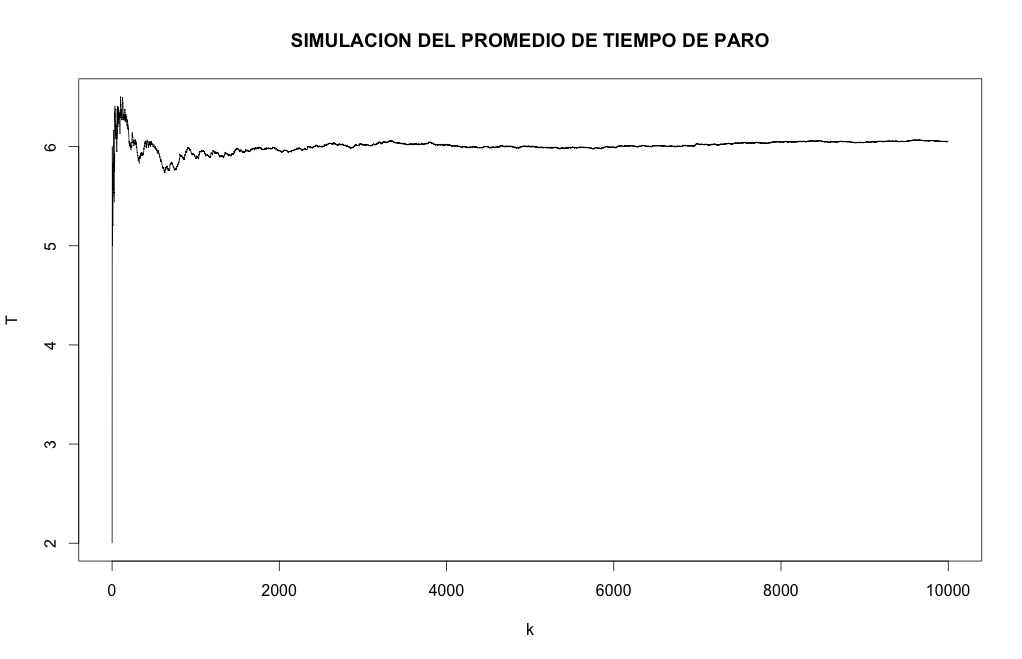
\includegraphics[width=0.7\textwidth]{simula.jpg}
  \caption{Grafica 1}
  \label{fig:ejemplo}
\end{figure}

\end{enumerate}
\textcolor[rgb]{0.2,0.5,0.7}{
\begin{problema}[Extensiones del teorema de paro opcional]
Sea \(M=\paren{M_n,n\in\na}\) una (super)martingala respecto de una filtraci\'on \(\paren{\F_n,n\in\na}\) y sean \(S\) y \(T\) tiempos de paro.
\begin{enumerate}
                \item Pruebe que \(S\wedge T\), \(S+T\) y \(S\vee T\) son tiempos de paro.
                \item Sea \begin{esn}\F_T=\set{A\in\F:A\cap\set{T\leq n}\in\F_n\text{ para toda } n}\end{esn}es una \(\sigma\)-\'algebra, a la que nos referimos como la \(\sigma\)-\'algebra detenida en \(\tau\). Comente qu\'e puede fallar si \(T\) no es tiempo de paro. Pruebe que \(T\) es \(F_T\)-medible. 
                \item Pruebe que si \(T\) es finito, entonces \(M_T\) es \(\F_T\)-medible.
                \item Pruebe que si \(S\leq T\leq n\) entonces \(\F_S\subset\F_T\). Si adem\'as \(T\) es acotado entonces \(X_S,X_T\in L_1\) y \begin{esn}\espc{M_T}{\F_S}\leq M_S.\end{esn}
                \item Si \(X=\paren{X_n,n\in\na}\) es un proceso estoc\'astico \(\paren{\F_n}\)-adaptado y tal que \(X_n\in L_1\) y tal que para cualesquiera tiempos de paro acotados \(S\) y \(T\) se tiene que \(\esp{X_S}=\esp{X_T}\) entonces \(X\) es una martingala. Sugerencia: considere tiempos de paro de la forma \(n\indi{A}+(n+1)\indi{A^c}\) con \(A\in\F_n\).
                	\item Pruebe que el proceso $M^T$ obtenido al detener a $M$ al instante $T$ y dado por $M^T_n=M_{T\wedge n}$ es una martingala respecto de $\paren{\F_{T\wedge n},n\geq 0}$ pero tambi\'en respecto de $\paren{\F_{n},n\geq 0}$. Sugerencia: basta probar el resultado respecto de $\paren{\F_n}$ y para esto es \'util el inciso anterior.
\end{enumerate}
\end{problema}
}
\defin{Solucion: }
\begin{enumerate}
	\item Demostraremos que $S \wedge T$, $S \vee T$ y  $S+ T$ son tiempos de paro
	\begin{itemize}
		\item Como $\set{S \wedge T \leq n}^{c}=\set{S \wedge T > n }=\set{S>n} \cap \set{T>n} \in \F_n$ entonces $ \set{S \wedge T \leq n} \in F_n$
		\item Como $\set{S \vee T \leq n} = \set{S\leq n} \cap 	\set{T \leq n} \in \F_n$ entonces   $\set{S \vee T \leq n}  \in \F_n$
		\item Notemos que 
		$$
		\set{S+T=n}=\bigcup_{k=0}^{n}\set{S=k,T=n-k}=\bigcup_{k=0}^{n}\set{S=i}	\cap\set{T=n-i}\in \F_n
		$$
	Por lo tanto en los tres casos hemos demostrado que se cumple la propiedad de tiempo de paro y como consecuencia cada una de estas tres funciones es una variable
	aleatoria pues son $\F$-medibles
	\end{itemize}
	\item Se demostrar\'a que $\F_{T}$ como se defini\'o es $\sigma$-algebra
	\begin{itemize}
		\item Claramente $\Omega \in \F_T$ pues  $\Omega \cap \set{T\leq n} =\set{T\leq n } \in \F_n$ pues $T$ es tiempo de paro
		\item $\F_T$ es cerrado bajo complementaci\'on pues; supongamos $A \in \F_{T}$ lo que implica por definici\'on que $\forall  n, A\cap\set{T\leq n} \in \F_n$, pero 
		como $\F_n$ es $\sigma$-algebra entonces $(A\cap\set{T\leq n})^c = A^c \cup \set{T >n} \in \F_n $. Luego al ser $T$ un tiempo de paro implica que  el evento
		$\set{T \leq n} \in \F_n$, por lo que interceptando estos dos \'ultimos evento de $\F_n$ tendr�amos que:
		$$
		 (A^c \cup \set{T >n} )\cap\set{T\leq n}=(A^c\cap \set{T \leq n})\cup(\set{T>n}\cap\set{T\leq n}) \in \F_n
		$$
		Pero como $\set{T>n}\cap\set{T\leq n}=\emptyset$, entonces se sigue que $(A^c\cap \set{T \leq n})\ \in \F_n$  y por tanto se concluye que $A^c \in \F_T$
		\item $\F_T$  es cerrado bajo uniones numerables. Sea $\set{A_k}$ una colecci\'on numerable de elementos en $\F_T$ y $n\in \mathds{N}$\\
		Como:
		$$
		\set{\bigcup_{k=1}^{\infty}A_{k}}\cap\set{T\leq n}=\bigcup_{k=1}^{\infty}\set{\set{A_{k}}\cap\set{T\leq n}}	\in \F_n
		$$
		De donde lo ultimo es consecuencia de que $A_{k} 	\in \F_n \forall n$. Por lo tanto se concluye que $\F_T$ asi definida es  $\sigma$-algebra\\
	\defin{Comentario: }  Si $T$ no fuera tiempo de paro la cerradura bajo complementaci\'on podr\'a fallar pues en la prueba se requiere que T sea tiempo de paro 
	para demostrar que $\F_T$ es cerrado bajo complementaci\'on.\\
	
	Ahora tambi\'en tenemos que probar que $T$ es $\F_T$-medible. Como T toma valores en $\mathds{N}\cup\set{\infty}$ entonces bastar\'ia probar que para una $k  \in \mathds{N}$ se tiene que el evento $\set{T\leq k} \in \F_T$. Pero como:
	
	$$
	\set{T\leq k}\cap\set{T\leq n}=\set{T\leq min\set{k,n}}	 \in \F_{n\wedge k} \subset \F_n  \forall n \in \mathds{N}
	$$
	Entonces se sigue por la definici\'on de $\F_T$ que el evento $\set{T\leq k} \in \F_T$ y por tanto $T$ es $\F_T$-medible 
          \end{itemize}
         \item Ahora se probar\'a que si $T$ es finito, entonces  la variable $M_{T}$ es $\F_T$-medible.  Al ser $T$ finito tenemos que existe $N$ tal que 	$T<N$, adem\'as como  en 
         este caso $M_{T}$ toma valores reales entonces hay  que probar  que el evento $\set{M_{T} \in A} \in \F_T$  con $ A \in \B_{\mathds{R}}$ un boreliano arbitrario. Como:
         $$
         \set{M_{T} \in A}=\bigcup_{i=0}^{N}\set{M_{T} \in A}	\cap \set{T=i} = \bigcup_{i=0}^{N}\set{M_i \in A}\cap\set{T=i} 
         $$
          Entonces, sea $n$ arbitrario en $\mathds{N}$: 
          $$
         \set{M_{T} \in A}\cap\set{T\leq n}=\paren{\bigcup_{i=0}^{N}\set{M_i \in A}\cap\set{T=i}}\cap\set{T\leq n}=\bigcup_{i=0}^{N\wedge n}\set{M_i \in A}\cap\set{T=i}
         $$
         Como est\'amos intersectando elementos de la $\sigma$-algebra $\F_{i}$  (recuerde que T es tiempo de paro y por tanto $\set{T=i}\in\F_i$)	 y dado que
         $i\leq n$ se sigue que todos los conjuntos que se unen e intersectan son elementos de la $\sigma$-algebra $\F_n$ por lo tanto hemos probado que 
         para toda $n$:
         $$
         \set{M_{T} \in A}\cap\set{T\leq n} \in \F_n \Rightarrow   \set{M_{T} \in A} \in \F_T
         $$
	Por lo tanto $M_T$ es $\F_T$ medible
	\item Primero probaremos que si $S < T$ entonces $\F_{S} \subset \F_{T}$. Sea $A \in \F_S$ P.D.  $A \in \F_T$. Como $A \in \F_S$ entonces por definici\'on de
	$\F_S$ sabemos que  para toda $n \in \mathds{N}$   el evento $A\cap\set{S\leq n} \in \F_n$ pero notando que $\set{T\leq n} \subset \set{S\leq n}$ pues 
	$S < T$ entonces:
	$$
	A\cap\set{T\leq n} = A\cap\set{T\leq n}\cap\set{S\leq n}=\paren{A\cap\set{S\leq n}}\cap\set{T\leq n}	\in \F_n
 	$$
	Lo ultimo se debe a que $T$ es tiempo de paro  y a que $\paren{A\cap\set{S\leq n}} \in \F_n$ por hip\'otesis. Por lo tanto
	$$
	A\cap\set{T\leq n} \in \F_n \forall n 
	$$
	De donde por definici\'on $A\in \F_T$ y por tanto  $\F_{S} \subset \F_{T}$.\\
	Si ahora suponemos que existe una cota para $T$, (Existe $n$ tal que $T\leq n$) entonces :
	$$
	M_T=\sum_{i=1}^{n}M_{i}\mathds{1}_{T=i}
	$$
	$$
	\esp{\abs{M_T}}\leq \sum_{i=1}^{n}\esp{\abs{M_{i}\mathds{1}_{T=i}}}\leq \sum_{i=0}^{n}\esp{\abs{M_{i}}} < \infty
	$$
	Y como $S <T$ entonces S tambi\'en es acotado y  an\'alogamente se probar\'ia que $\esp{\abs{M_S}} < \infty$ de donde se concluye que 
	$M_{S},M_{T} \in \mathds{L}_1$\\
	Resta probar que $\esp{M_{T}|\F_{S}}\leq M_{S}$. Probaremos primero la igualdad. Para demostrar que la $M_S$ es una versi\'on de la esperanza condicional hay que verificar 	dos cosas:
	\begin{itemize}
		\item $M_S$ es $\F_S$ medible lo cual ya se hab\'ia probado en el inciso (2) (S\'olo hay  que cambiar T por S en la demostraci\'on)
		\item $\esp{M_{T}\mathds{1}_{A}}=\esp{M_{S}\mathds{1}_{A}}$ para toda $A \in \F_S$ .\\ Para demostrar esto \'ultimo expres\'amos a $M_{T}-M_{S}$ como una suma 					telesc\'opica de la siguiente forma:
		$$
		M_T-M_S=\sum_{i=0}^{n}\paren{M_i-M_{i-1}}\mathds{1}_{S<i\leq T}
		$$
		Tomamos $A \in F_S$ arbitrario  por lo que $A\cap \set{S\leq n} \in \F_n$ para toda $n$. Luego multiplicando la expresi\'on anterior por $\mathds{1}_A$ y tomando 				esperanza
		$$
		\esp{\paren{M_T-M_S}\mathds{1}_A}=\esp{\sum_{i=0}^{n}\paren{M_i-M_{i-1}}\mathds{1}_{\set{S<i\leq T}}\mathds{1}_A}
		$$
		Como $\mathds{1}_{\set{S<i\leq T}}\mathds{1}_A=\mathds{1}_{\set{S<i}\cap A} \mathds{1}_{i\leq T}$. Pero por hip\'otesis $\set{S<i}\cap A \in \F_{i-1}$ y dado que $T$ es un 		tiempo de paro  $\set{i\leq T}=\set{T\leq i-1}^c 	\in \F_{i-1}$
		$$
		\esp{\sum_{i=0}^{n}\paren{M_i-M_{i-1}}\mathds{1}_{\set{S<i\leq T}}\mathds{1}_A}=\sum_{i=0}^{n}\esp{\paren{M_i-M_{i-1}}\mathds{1}_{\set{S<i\leq T}}\mathds{1}_A}
		$$
		$$
		=\sum_{i=0}^{n}\esp{\esp{\paren{M_i-M_{i-1}}\mathds{1}_{\set{S<i}\cap A} \mathds{1}_{i\leq T}|\F_{i-1}}}
		$$
		$$
		=\sum_{i=0}^{n}\esp{\mathds{1}_{\set{S<i}\cap A}\esp{\paren{M_i-M_{i-1}}|\F_{i-1}} \mathds{1}_{i\leq T}}=0
		$$
	         Pues las ser $M_i$ martingala   se tiene que 
	         $$
	         \esp{\paren{M_i-M_{i-1}}|\F_{i-1}}=M_{i-1}-M_{i-1}=0  
	         $$
	         De donde concluimos que para todo $A \in \F_S$  se tiene que:
	         $$
	         \esp{\paren{M_T-M_S}\mathds{1}_{A}}=0  \Longleftrightarrow  \esp{M_T\mathds{1}_A}=\esp{M_S\mathds{1}_A}
	         $$ 
		Por lo tanto 
		$$
		\esp{M_{T}|\F_{S}}=M_{S} \text{ casi seguramente}
		$$
		La prueba con la desigualdad es an\'aloga solo hay que notar que ahora supondr�amos que estamos con una supermartingala y por tanto
		$$
		   \esp{\paren{M_i-M_{i-1}}|\F_{i-1}}\leq 0
		$$
		
		
	
	\end{itemize}
	
	
	
	\item Hay que probar que X=$\paren{X_n, n\in \mathds{N}}$ es martingala, por lo tanto hay que probar tres cosas
	\begin{itemize}
		\item $X_n$ es adaptado por construcci\'on entonces $X_n$ es $\F_n$-medible
		\item $X_n \in \mathds{L}_{1}$ por como se defini\'o el proceso $X$
		\item S'olo resta demostrar que $\esp{X_{n+1}|\F_n}=X_{n}$\\	
		Para demostrarlo usaremos la sugerencia y definiremos el tiempo de paro $T_n=\mathds{1}_{A}+(n+1)\mathds{1}_{A^c}$ con $A \in {\F_n}$ arbitrario.\\
		Haremos unas observaciones
		\begin{itemize}
			\item $T_n$ asi definido es tiempo de paro pues el evento $\set{T_n=k} \in \F_k$  para toda $k$. En efecto pues $\set{T_n=k}=\emptyset$ si $k \notin \set{n,n+1}$
				; $\set{T_n=n}=A \in \F_n$  y $\set{T_n=n+1}=A^c \in \F_n$ 
			\item $T_n$  solo toma dos valores :$n$ y $n+1$; por lo que es un tiempo de paro acotado por $n+1$
		\end{itemize}
		Por otro lado definamos el tiempo de paro constante $S_n=n+1$ (Es tiempo de paro por ser medible para cualquier $\sigma$-\'algebra) el cual tambi\'en es acotado. 
		Entonces por ser $T_n$ y $S_n$ tiempo de paros acotados se tendr\'ia que por hip\'otesis $\esp{X_{T_n}}=\esp{X_{S_n}}$ \\
		Con estas dos definiciones tenemos lo siguiente:
		$$
		X_{T_n}=\sum_{i=0}^{\infty}X_{i}\mathds{1}_{T=i}=X_n\mathds{1}_{T=n}+X_{n+1}\mathds{1}_{T=n+1}=X_n\mathds{1}_{A}+X_{n+1}\mathds{1}_{A^c}
		$$
		Por lo tanto para cualquier $A	\in \F_n$ se tendr�a:
		$$
		\esp{X_{T_n}}=\esp{X_n\mathds{1}_{A}+X_{n+1}\mathds{1}_{A^c}}=\esp{X_n\mathds{1}_{A}}+\esp{X_{n+1}\mathds{1}_{A^c}}
		$$
		y  como $S_n=n+1$ entonces
		$$
		 \esp{X_{S_n}}=\esp{X_{n+1}}=\esp{X_{n+1}\mathds{1}_{A}+X_{n+1}\mathds{1}_{A^c}}=\esp{X_{n+1}\mathds{1}_{A}}+\esp{X_{n+1}\mathds{1}_{A^c}}
		$$
		y recordando que \esp{X_{S_n}}=\esp{X_{T_n}}  se tendr\'ia que:
		$$
		\esp{X_{n+1}\mathds{1}_{A}}+\esp{X_{n+1}\mathds{1}_{A^c}}=\esp{X_n\mathds{1}_{A}}+\esp{X_{n+1}\mathds{1}_{A^c}}
		$$
		Entonces:
		$$
		\esp{X_n\mathds{1}_{A}}=\esp{X_{n+1}\mathds{1}_{A}}
		$$	
		Notemos que la anterior igualdad es para todo $A\in \F_n$ y recordando la definici\'on de Esperanza condicional  tend�amos que $X_n$ es una representaci\'on 
		de  $\esp{X_{n+1}|\F_n}$. Pues 
		\begin{itemize}
			\item $X_n$ es $\F_n$-medible
			\item  $\esp{X_n\mathds{1}_{A}}=\esp{X_{n+1}\mathds{1}_{A}} \forall A \in \F_n$
		\end{itemize}
		
		De donde se sigue que:
		$$
		\esp{X_{n+1}|\F_n}=X_{n}	  \text{ casi seguramente}
		$$
		Por lo tanto X=$\paren{X_n, n\in \mathds{N}}$ es martingala
		
	\end{itemize}
	 
	 \item  Para probar que $M_n^T$ es martingala  utilizaremos el ejercicio anterior.  Tenemos pues un proceso estoc\'astico  $M_n^T$ que es claramente $\F_n$ - adaptado, pues como $T \wedge n \leq n$ entonces:
	 $$
	  M_n^T=\sum_{k=1}^{n}M_i\mathds{1}_{T\wedge n=i}
	 $$ 
	De donde se concluye que $M_n^T$ es $\F_n$ medible para toda $n$.\\
	Por otro definamos dos tiempos de paro acotados $T\wedge n$ y $S\wedge n$  arbitrarios. Como $M_n$ es martingala  entonces usando el Muestreo opcional del Doob en los dos tiempos de paro definidos obtenemos;
	$$
	\esp{M_{T\wedge n}}=\esp{M_1}=\esp{M_{S\wedge n}}
	$$	
	
	Por lo tanto $\esp{M_{T\wedge n}}=\esp{M_{S\wedge n}}$ de donde usando el ejercicio anterior concluimos que $M_n^T$ es martingala.
	
	
	
	
	
	
\end{enumerate}

\bibliography{GenBib}
\bibliographystyle{amsalpha}
\end{document}